% !TeX encoding = UTF-8
% !TeX spellcheck = en_US
% !TeX root = presentation.tex
% !TeX TS-program = xelatex
% !BIB TS-program = biber

\documentclass[showdate=true, slidenumbers=slide]{beamerruhuisstijl169}

\usepackage{fontspec}
\setsansfont[
    Path = ./fonts/,
    Extension = .otf,
    BoldFont = *-Bold,
    BoldItalicFont = *-BoldItalic,
    ItalicFont = *-Italic,
    UprightFont = *-Regular
]{Inter}

\setmonofont[
    Path = ./fonts/,
    Extension = .ttf,
    BoldFont = *-Bold,
    BoldItalicFont = *-BoldItalic,
    ItalicFont = *-Italic,
    UprightFont = *-Regular
]{RobotoMono}

\usepackage{xcolor}
\usepackage{appendix}

\usepackage{graphicx}

\usepackage{listings}

\definecolor{codegreen}{rgb}{0,0.6,0}
\definecolor{codegray}{rgb}{0.5,0.5,0.5}
\definecolor{codepurple}{rgb}{0.58,0,0.82}
\definecolor{backcolour}{rgb}{0.95,0.95,0.92}

\lstdefinestyle{mystyle}{
    backgroundcolor=\color{backcolour},
    commentstyle=\color{codegreen},
    keywordstyle=\color{magenta},
    numberstyle=\tiny\color{codegray},
    stringstyle=\color{codepurple},
    basicstyle=\ttfamily\footnotesize,
    breakatwhitespace=false,
    breaklines=true,
    captionpos=b,
    keepspaces=true,
    numbers=left,
    numbersep=5pt,
    showspaces=false,
    showstringspaces=false,
    showtabs=false,
    tabsize=2
}
\lstset{style=mystyle}

\title{Testing Techniques}
\subtitle{Group 5 - Testing the Transmission Control Protocol (TCP)}
\date{\today}
\author{Nikolay Kyosev \and David Oberacker \and Bram Pellen \and Orpheas van Rooij}

\begin{document}

\begin{frame}
    \maketitle
\end{frame}

\begin{frame}
    \tableofcontents
\end{frame}

\section{System Under Test}

\begin{frame}{TCP}

\end{frame}

\section{Test Architecture}

\begin{frame}{Test Architecture}
    \centering
    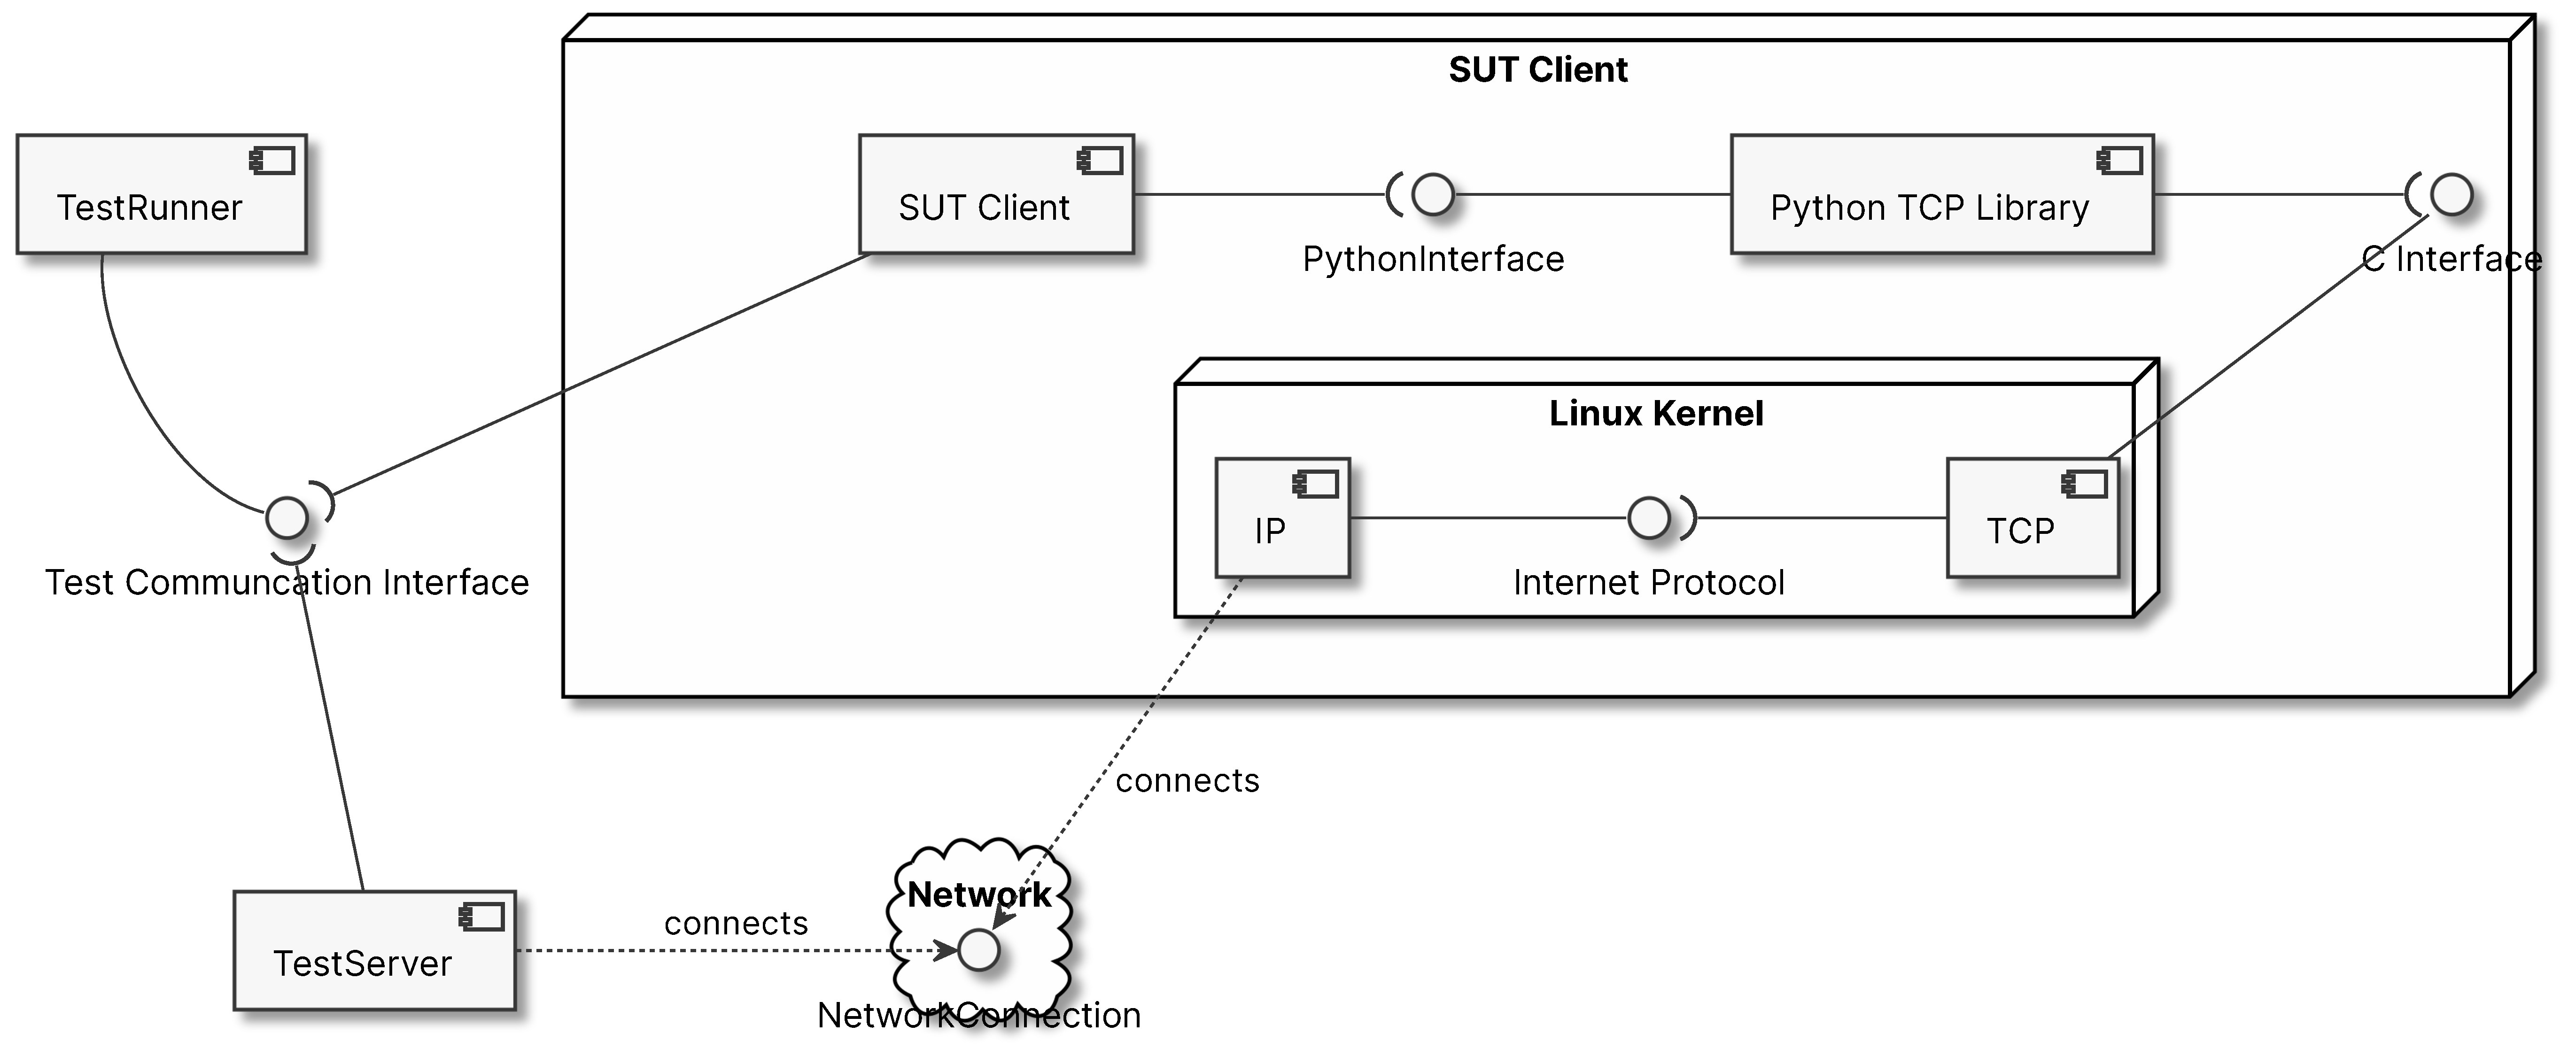
\includegraphics[width=\textwidth]{figures/SUTArchitecture.pdf}
\end{frame}

\begin{frame}{SUT Client}
    \begin{itemize}
        \item 3 Sub-components
        \item \textbf{SUT client}
        \begin{itemize}
            \item Test management functions
            \item Result checks
            \item Mocking of user calls
            \item Reports results to the TestRunner
        \end{itemize}
        \item \textbf{TCP Kernel implementation}
        \begin{itemize}
            \item Our actual System Under Test
            \item Uses the IP interface
            \item Interfaced using C functions
        \end{itemize}
        \item \textbf{Internet Protocol (IP) implementation}
        \begin{itemize}
            \item Communication with the \textbf{TestServer}
        \end{itemize}
    \end{itemize}
\end{frame}

\begin{frame}{Test Server}
    \begin{itemize}
        \item Represents the \textbf{SUT}s communications partner
        \item Does not use a TCP implementation
        \item Verifies incoming packages
        \begin{itemize}
            \item Comparisons against expected values
        \end{itemize}
        \item Creates reply packages
        \begin{itemize}
            \item Field values have to be specified
            \item Some automation for e.g. \textit{sequence numbers}
        \end{itemize}
        \item Reports to the \textbf{TestRunner}
        \item Depends on the IP protocol
    \end{itemize}
\end{frame}

\begin{frame}{Test Runner}
    \begin{itemize}
        \item Test management component
        \begin{itemize}
            \item Loads test case files
            \item Controls test execution
            \item Does not evaluate actual results
        \end{itemize}
        \item Sends instructions to \textbf{TestServer} and \textbf{SUT Client}
        \begin{itemize}
            \item Uses a DSL for specifying inputs and expected results
            \item Only checks that DSL command exit status
            \item Collects tracing information from reply's
        \end{itemize}
        \item Uses TCP Websockets for communication
    \end{itemize}
\end{frame}

\begin{frame}{Command Language}
    \begin{columns}[T,totalwidth=\linewidth]
        \begin{column}{0.5\textwidth}
            \begin{itemize}
                \item JSON based DSL
                \item \texttt{testNumber} for test case identification
                \item Different command types
                \begin{itemize}
                    \item \textit{SendReceive} - Sends package \& expect reply
                    \item \textit{Connect} - Perform a TCP handshake
                    \item \textit{Receive} - Expect incoming package
                    \item \dots
                \end{itemize}
                \item Specific parameters per \texttt{commandType}
            \end{itemize}
        \end{column}
        \begin{column}{0.5\textwidth}
            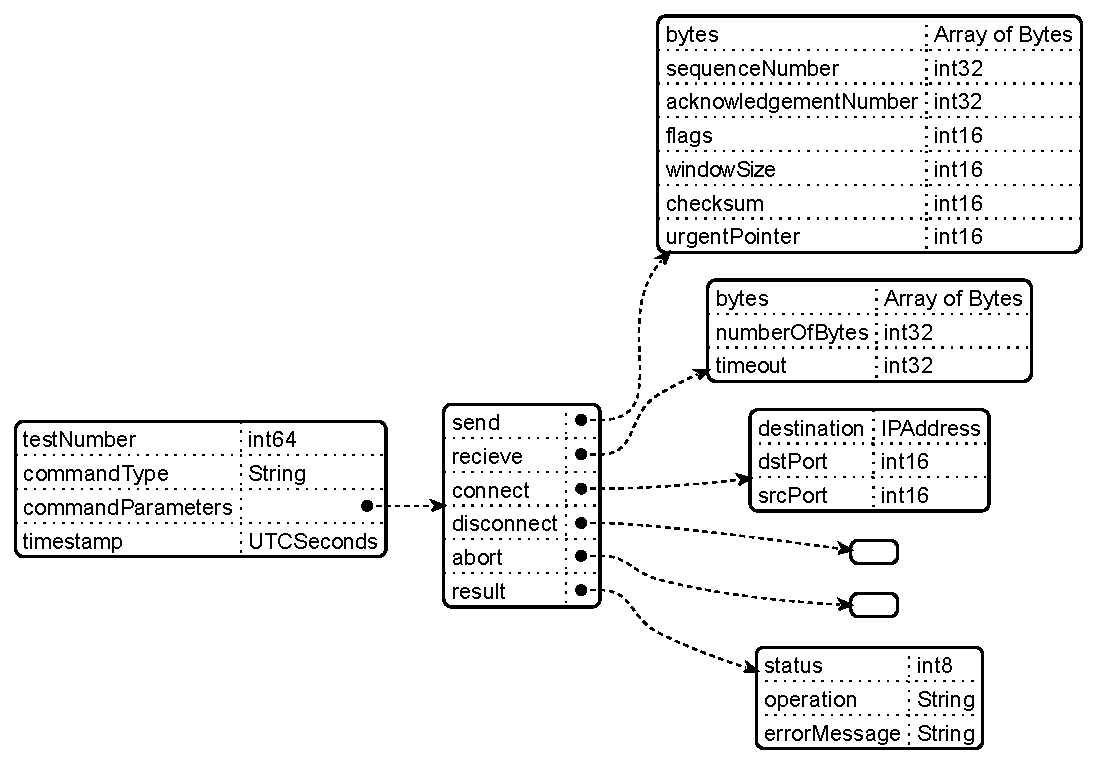
\includegraphics[width=\textwidth]{figures/ControlMessagesJson.pdf}
        \end{column}
    \end{columns}
\end{frame}

\begin{frame}{Test Case Definition}
    \begin{columns}[T,totalwidth=\linewidth]
        \begin{column}{0.6\textwidth}
            \begin{itemize}
                \item Consists of two phases
                \begin{itemize}
                    \item \textbf{Initialization phase}
                    \item \textbf{Test phase}
                \end{itemize}
                \item Commands are always verified
                \begin{itemize}
                    \item Initialization phases are explicitly covered
                \end{itemize}
                \item Special commands for synchronization
                \begin{itemize}
                    \item \textit{Sync} - Wait until SUT \& Test server reach this point
                    \item \textit{Wait} - Wait time until sending the next command
                \end{itemize}
                \item Specified as UML sequence diagrams
                \item Total of 14 test cases defined
            \end{itemize}
        \end{column}
        \begin{column}{0.4\textwidth}
            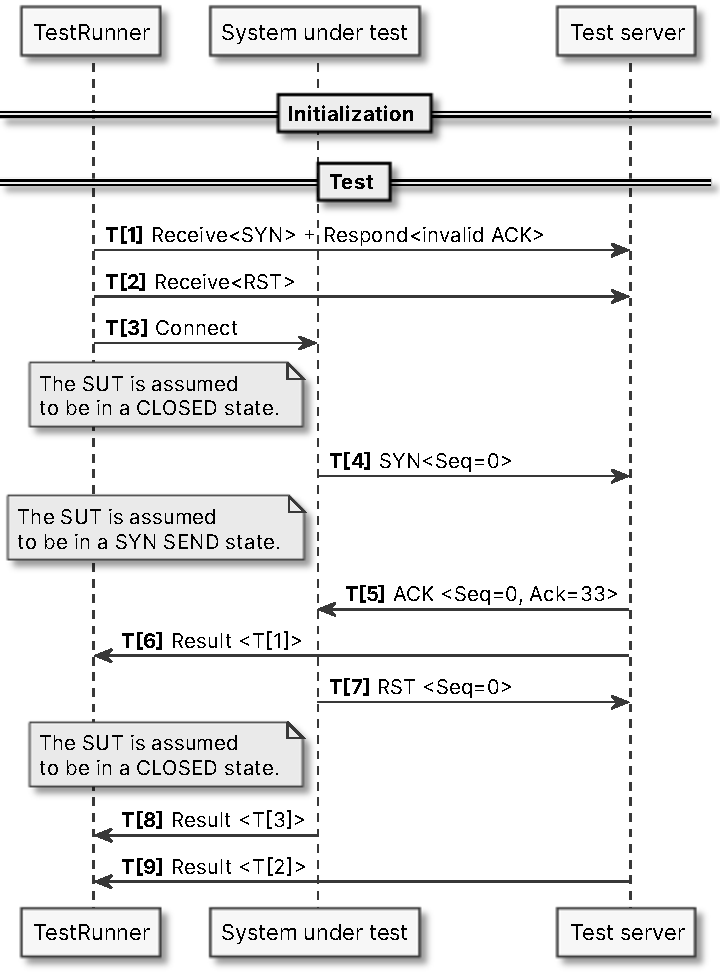
\includegraphics[height=0.75\textheight]{figures/testcases/TestCase3.pdf}
        \end{column}
    \end{columns}
\end{frame}

\begin{frame}{Test Case Implementation}
    \lstinputlisting[language=Python, firstline=33, lastline=45]{figures/test3.py}
\end{frame}

\section{Test Implementation \& Results}

\section{Model Based Testing}

\begin{frame}
\vfill
\centering
{\LARGE Thank you for your attention.}\\
\vspace{1cm}
{\Large \textbf{Questions ?}}
\vfill
\end{frame}

\appendix
\begin{frame}{Disclaimer}
    \begin{block}{Introduction}
        This presentation shows the possibilities of the Beamer version of the Radboud University's new (2014) corporate style Powerpoint template. Note that although one of the parameters to the document class for Beamer is \texttt{official}, and the university encourages the use of this template, only the Powerpoint and Keynote templates are officially supported. See \url{http://www.ru.nl/huisstijl/} for everything corporate style related.
    \end{block}

    \begin{block}{Questions, feedback, and comments}
        Don't hesitate to contact me, also if you have questions on how to realise certain parts of your presentation.
        \begin{description}
            \item[Email] \href{mailto:l.onrust@let.ru.nl}{l.onrust@let.ru.nl}
            \item[Github] \href{https://github.com/naiaden}{naiaden}
        \end{description}
    \end{block}
\end{frame}

\begin{frame}{Distribution and Availability}
    \begin{block}{Availability}
        The code of the Beamer class file and the background images are hosted at github: \url{https://github.com/naiaden/presentations/tree/master/ruhuisstijl/distributed}. There you will always find the newest version.

        The template on \textbf{write}\LaTeX{} is updated after every push to github. It may take a couple of days before the administrators of \textbf{write}\LaTeX{} approve the new version of the template.
    \end{block}

\end{frame}

\begin{frame}{Usage}
    \begin{block}{How to use this template}
        To use this template for your own presentation in \textbf{write}\LaTeX{}, perform the next steps:
        \begin{enumerate}
            \item remove all frames in the \texttt{tex} file;
            \item enable only the options that you want to use (because right now it is in handout-mode with 2 slides and their notes on a page, with a departmental layout);
            \item create frames with your slide's content;
            \item thoroughly look everything over, and check for overflows, wrong spacing after interpunction, spelling. \emph{everything}.
        \end{enumerate}
    \end{block}

    \begin{block}{Title page}
        The creators of the official corporate style chose to have only a title and subtitle field on the title page. If you want to put all sorts of extra information there, I don't mind, but you are on your own.
    \end{block}
\end{frame}

\begin{frame}{Structure of this Presentation}
    This presentation consists of three parts:
    \begin{columns}[T,totalwidth=\linewidth]
        \begin{column}{0.3\textwidth}
            \begin{block}{Voorbeeldpresentatie}
                Here we recite the rules as stated in the \href{http://www.ru.nl/publish/pages/596464/ru_powerpoint_algemeen_2014_toelichting.ppt}{example presentation}. This section is in Dutch
            \end{block}
        \end{column}
        \begin{column}{0.3\textwidth}
            \begin{block}{Examples}
                Here we show tricks such as \texttt{uncover}, \texttt{only}, smart references, and nested lists.
            \end{block}
        \end{column}
        \begin{column}{0.3\textwidth}
            \begin{block}{Showcase}
                Here we demonstrate the possible departmental styles, both the title page and the layout for the slides.
            \end{block}
        \end{column}
    \end{columns}

    \begin{block}{Additional comments}
        Each frame (not necessarily each slide) has a note. Pass \texttt{show notes} as an option to the document class to show them, or look in the code. In the notes I will provide some thoughts and explanations.
    \end{block}
\end{frame}

\setbeamercolor{title}{fg=ruhuisstijlzwart}

\section{Voorwaarden}
\subsection{Algemeen}
\begin{frame}\label{sl:gvwa}
    \frametitle{Gebruiksvoorwaarden algemeen}

    \begin{block}{Titelpagina's (rood)}
        \begin{itemize}
            \item Maak altijd gebruik van de rode titelpagina met het logo van de Radboud Universiteit rechtsonder
            \item Er mogen geen extra tekstvelden of afbeeldingen worden toegevoegd
            \item Indien een openingspagina als tussenpagina wordt gebruikt mogen er wel afbeeldingen toegevoegd worden
        \end{itemize}
    \end{block}

    \begin{block}{Tekstpagina's}
        \begin{itemize}
            \item Gebruik voor tekstpagina's altijd de witte dia met het logo in de rode balk
            \item Teksten linkslijnend plaatsen, niet centreren
        \end{itemize}
    \end{block}
\end{frame}

\subsection{Tekstpagina's}
\begin{frame}{Gebruiksvoorwaarden titelpagina's (rode achtergrond)}
    \begin{block}{Maak altijd gebruik van lettertype Arial}
        \begin{itemize}
            \item Paginatitel: standaard, 50 pt
            \item Tekst/inhoud: standaard, 25 pt
        \end{itemize}
    \end{block}

    \begin{block}{Plaats teksten altijd in zwart of wit}
        \begin{itemize}
            \item Paginatitel: wit
            \item Inhoud tekst: zwart
        \end{itemize}
    \end{block}

    \begin{block}{Maak altijd gebruik vastgestelde kantlijn}
        \begin{itemize}
            \item Titel en tekst/inhoud: horizontaal vanaf links 2,5 cm
            \item Titel: verticaal vanaf boven 2 cm
            \item Tekst/inhoud: verticaal vanaf boven 5 cm
        \end{itemize}
    \end{block}
\end{frame}

\begin{frame}
    \frametitle{Gebruiksvoorwaarden tekstpagina's (witte achtergrond)}

    \begin{block}{Maak altijd gebruik van lettertype Arial}
        \begin{itemize}
            \item Paginatitel: standaard, grootte 30 pt
            \item Tekst/inhoud: standaard, grootte 25 pt (of 21 pt)
            \item Tussenkoppen: vet, grootte 25 pt (of 21 pt)
            \item Fotobijschriften: standaard, grootte 18 pt
        \end{itemize}
    \end{block}

    \begin{block}{Plaats teksten altijd in zwart of rood}
        \begin{itemize}
            \item Paginatitel: RU huisstijl rood {\color{ruhuisstijlrood} (RGB: 190, 49, 26)}
            \item Inhoud tekst en tussenkoppen: zwart
        \end{itemize}
    \end{block}

    \begin{block}{Maak altijd gebruik vastgestelde kantlijn}
        \begin{itemize}
            \item Titel en tekst/inhoud\footnote{Afbeeldingen en teksten mogen nooit over de onderste lijn en het logo geplaatst worden.}
            : horizontaal vanaf links 2,5 cm
            \item Titel: verticaal vanaf boven 2 cm
            \item Tekst/inhoud: verticaal vanaf boven 5 cm
        \end{itemize}
    \end{block}

\end{frame}

\section{Kleuren}
\begin{frame}
    \frametitle{Kleuren in het RU Thema}

    Zwart: RGB 0/0/0 \\
    Wit: RGB 250/250/250 \\
    \rured{Rood: RGB 190/49/26 (RU huisstijl rood)} \\
    \href{http://google.com/}{Hyperlink: RGB 190/49/26 (RU huisstijl rood)}
\end{frame}

\section{Sjablonen}
\begin{frame}
    \frametitle{Sjablonen}

    \begin{block}{}
        Alle gebruikte sjablonen zijn aangemaakt in het basisdocument. \\
        U vindt de sjablonen onder Dia's > indelingen.
    \end{block}

    \begin{block}{}
        Gebruik sjablonen uit de mappen:
        \begin{itemize}
            \item Dia's > Indelingen > \rured{RU Tekstpagina's}
            \item Dia's > Indelingen > \rured{RU Titelpagina's}
        \end{itemize}
    \end{block}

    \footnotetext{Hierna volgen enkele voorbeeldpagina's, de paginatitels zijn gelijk aan de naam van het sjabloon}

\end{frame}


\section{Voorbeeldslides}

\subsection{Blokken}
\begin{frame}{Titel en object}
    \begin{block}{Dit is een tussenkop}
        Rectiatem sunto bla velesti berestrupta conseria quam quae commo et eaquam quo dolent omnistis estion cuptatet duciendae dolorunt ipit, omnimus trumqui ommolor simporuntium fugit eicatem quis autem eatemquiam nissum eatum facerit inciis voluptas quae aut et es dellab ipsum, ium alis aboriandunt ea sinverios sequo ea consedi psapid.
    \end{block}

    \begin{block}{}
        Een opsomming:
        \begin{itemize}
            \item que volore non etur aut laborum, te repudam, sus es acerrov itatest omnitatur, ea vid qui tempore re, alique.
            \begin{itemize}
                \item Am restibusam nihillor
                \item Alias ne officati officate
                \item Sequae dollitate porat vitatem
            \end{itemize}
        \end{itemize}
    \end{block}
\end{frame}

\begin{frame}{Twee objecten}
    \begin{columns}[T,totalwidth=\linewidth]
        \begin{column}{0.475\textwidth}
            \begin{block}{Dit sjabloon kunt u gebruiken voor twee tekstkolommen}
                Berestrupta conseria quam quae commo et eaquam quo dolent omnistis estion cuptatet duciendae ommolor simporuntium fugit eicatem quis autem eatemquiam nissum eatum facerit inciis voluptas quae
                aut et es dellab ipsum, ium alis aboriandunt ea sinverios sequo ea consedi psapid molore autestium dio el in pelibea rcimustio esectae moluption reriam.
            \end{block}
        \end{column}
        \begin{column}{0.475\textwidth}
            \begin{block}{}
                Am restibusam nihillor alias ne officati officate numet, quiate autem rerro ipsam, sequae dollitate porat vitatem litatiaestis acesequid et ut moluptas dolorum voluptat a poruntibus imillaut fugia velitatempor.
            \end{block}
            \begin{block}{}
                Magniscil illuptibus moleceria cumquis doluptu saerro in coresto volorecesse modit qui omnima volluptur, quo magnia coratis dus et faccae non plibusant. Ugit voluptatio eseria possimaio opturitatur.
            \end{block}
        \end{column}
    \end{columns}
\end{frame}

\begin{frame}{Vergelijking}
    \begin{columns}[T,totalwidth=\linewidth]
        \begin{column}{0.5\textwidth}
            \begin{block}{Sapienis simet esto ugit voluptatio eseria possimaio opturitatur}
                \begin{itemize}
                    \item Nem aut aut ipsa nest volo doluptat vendelique nimus simossi.
                    \item Magnihi cimaios descidist verum, con rere que molenis adipsus apisin repressunt atibuscipsum.
                    \item Velibust praestiore natur, coresed que que dolut raturer roreperciae veribus num voloreiciet arum que.
                    \item Quatemped unt la dolores sequodi gnataes dictibus estrunt iorers pedia de pelluptae.
                \end{itemize}
            \end{block}
        \end{column}
        \begin{column}{0.5\textwidth}
            \begin{block}{Imus acerita dis quasper lita tiaestis acesequid et ut moluptas}
                \begin{itemize}
                    \item Quisqui aut aut volutem quam quo tet, quam iliquiatqui conseque dita
                    \item Aut harum ipsam vid untia ne dolupta corum de qui.
                    \item Aut qui ut utet everrum quatur sunto ea sunt lam que sae lit aut volupta turerum exeri.
                    \item Dolorit odi utemqui coris magnatus experfe rionsequam rera vel mil maiorupta serae dolupiet ius aliciti simagnimodi.
                \end{itemize}
            \end{block}
        \end{column}
    \end{columns}
\end{frame}

\subsection{Tabel}
\begin{frame}\label{sl:vvet}
    \frametitle{Voorbeeld van een tabel}

    \begin{tabular}{=l +r +r +r +r }
        \rowcolor{ruhuisstijlrood}\rowstyle{\color{white}} & Kolom 1 & Kolom 2 & Kolom 3 & Kolom 4 \\
        Rij 1 & 101 & 201 & 301 & 401 \\
        Rij 2 & 102 & 202 & 302 & 402 \\
        Rij 3 & 103 & 203 & 303 & 403 \\
        Rij 4 & 104 & 204 & 304 & 404 \\
        Rij 5 & 105 & 205 & 305 & 405 \\
        \rowstyle{\color{ruhuisstijlrood}}Totaal & 515 & 1015 & 1515 & 2014
    \end{tabular}
\end{frame}

\subsection{De rest}
\begin{frame}{Niet alles blootgeven}
    De \pause tekst \pause verschijnt \pause in \pause stukken.\footnote{Voetnoottest.}\footnote{Soms zijn er meerdere voetnoten.}

    \begin{itemize}
        \item<+-> dit verschijnt pas als ``stukken.'' getoond is
        \item<+-> dit verschijnt van de tweede actie tot het einde
        \item<+-+> dit verschijnt eenmalig van de derde tot de vierde actie
        \item<-+> Dit zal er staan vanaf het begin tot de vijfde actie.
        \item<+-> Dit zal er op het einde komen
    \end{itemize}
\end{frame}

\begin{frame}{Nog een ander voorbeeld met stappen}
    Alert kan \alert<+->{ook}
    \emph<+->{andere} dingen:

    \uncover<+->{ zoals}
    \visible<+->{ dit}
    \only<+->{ leuke}
    trucje
\end{frame}

\begin{frame}{Hebban olla vogala nestas hagunnan hinase hic anda thu?}
    \begin{itemize}
        \item Wat unbidan we nu
        \begin{itemize}
            \item Habent omnes uolucres nidos inceptos nisi ego et tu. Quid expectamus nunc.
            \begin{itemize}
                \item Have all birds begun nests, except me and you, what are we waiting for?
                \item Es haben alle V\"ogel Nester begonnen, nicht aber ich und du, was wartet Ihr nun?
            \end{itemize}
        \end{itemize}
        \item De tekst, die werd geschreven door een West-Vlaamse kopiist,
        \item dateert naar schatting uit het derde kwart van de 11e eeuw.
        \item  De eerste twee zinnen zijn in het Latijn.
        \item De taal waarin de rest van de tekst geschreven is wordt door de meeste taalkundigen als Oud-Westnederfrankisch aangeduid
        \item maar hierover bestaat nog controverse.
    \end{itemize}
\end{frame}

\begin{frame}{Hier tellen we mee}
    Eerst maar eens de kantlijn bepalen.
    \begin{enumerate}
        \item Tel je mee?
        \item De tweede
        \item Drie!
        \begin{enumerate}
            \item Drie-en-een-beetje
            \item Drie-en-half
            \item \label{haha} Twee ei is geen ei
        \end{enumerate}
        \item Vier!!!!!
    \end{enumerate}

    H\'e, \ref{haha} hoort daar helemaal niet.

    \begin{description}
        \item[Een item] Ook de description maar even testen met een veel-te-lange regel om te kijken wat er dan gebeurt.
        \item[Mag] ook kort zijn uiteraard.
        \item[Maar wat nu als] het label van zichzelf wel erg lang is?
    \end{description}
\end{frame}

\begin{frame}{Opsommingen enzo}
    Eerst even wat normale tekst om de kantlijn te bepalen.
    \begin{itemize}
        \item[$\star$] Item 0
        \item Dit is item 1
        \begin{itemize}
            \item Dit is een ander item 1.1
            \item[$\Gamma$] Een \emph{custom} item 1.2
            \begin{itemize}
                \item $\alpha \beta \gamma$
                \item Maak deze regel dan maar gewoon lekker lang om te zien hoe de indentatie is.
            \end{itemize}
        \end{itemize}
        \item Item 2 dan maar
    \end{itemize}

    \begin{enumerate}
        \item First item
        \begin{enumerate}
            \item Nested.
        \end{enumerate}
    \end{enumerate}
\end{frame}

\begin{frame}{Ander soort van opsomming}
    \[ a+b=4 \]

    \begin{equation}
        \begin{split}
            a = 2 \\
            b = 2
        \end{split}
    \end{equation}

\end{frame}

\begin{frame}{Tips}
    \begin{block}{Handout}
        Als je in de preamble \texttt{handout} als optie aan de documentclass \texttt{beamerruhuisstijl} meegeeft, dan maakt hij per slide 1 pagina aan. Ook al gebruik je overlays en stapsgewijze opsommingen.
    \end{block}

    \begin{block}{Inhoudsopgave per sectie}
        Als je superveel te vertellen hebt, maak dan een slide aan met een inhoudsopgave van het hoofdstuk wat je op dat moment gaat beginnen met \texttt{\textbackslash tableofcontents[currentsection]}
    \end{block}

    \begin{block}{Notities voor op het tweede scherm}
        Net als de presenter view van PowerPoint, kun je met \texttt{beamer} ook notities maken. Zoek in de source code maar op \texttt{\textbackslash note}. Standaard staan ze aan, maar als je na je frame niet aangeeft dat je notes wilt, dan wordt er ook geen pagina voor aangemaakt.
    \end{block}
\end{frame}

\begin{frame}{De \'echt onoffi\"ele opties}
    \begin{block}{Tabellen}
        \texttt{tablecolours}: false, true. Als true, dan alterneren de rijen van kleur.
    \end{block}

    \begin{block}{Titelpagina}
        \texttt{showinstitute}: false, true (default = false). Als true dan wordt ook je institute opgenomen op de titelpagina.
        \texttt{showdate}: false, true (default = false). Als true dan wordt ook de datum opgenomen op de titelpagina.
    \end{block}

    \begin{block}{Overzicht}
        \texttt{slidenumbers}: none, slide, relative (default = none). Toon slidenummer in voetlijn; relatief is bijvoorbeeld 4/21.
        \texttt{alwaysshowauthor}: false, true (default = false). Toon auteur in voetlijn.
        \texttt{alwaysshowdate}: false, true (default = false). Toon datum in voetlijn.
        \texttt{tocatsectionstart}: false, true (default = false). Begin elke section met een inhoudsopgave met de titel \texttt{tocatsectionstarttitle}.
    \end{block}
\end{frame}


\end{document}